\documentclass[a4paper,12pt,french]{article}
\usepackage[margin=2cm]{geometry}
\usepackage[thinfonts]{uglix2}
\nouveaustyle
\begin{document}
\titre{CH01 - Exercices}{NSI2}{09/2021}

\begin{encadrecolore}{Activité préparatoire}{UGLiOrange}
Te rappelles-tu ce qu'est une poignée de main ? Voici comment \textsc{Wikipédia} définit cette coutume « pré-Covid 19 »:\\
\textit{Une poignée de main est un geste de communication effectué le plus souvent en guise de salutation mais qui peut également être une signification de remerciement ou d'accord.}
\begin{center}
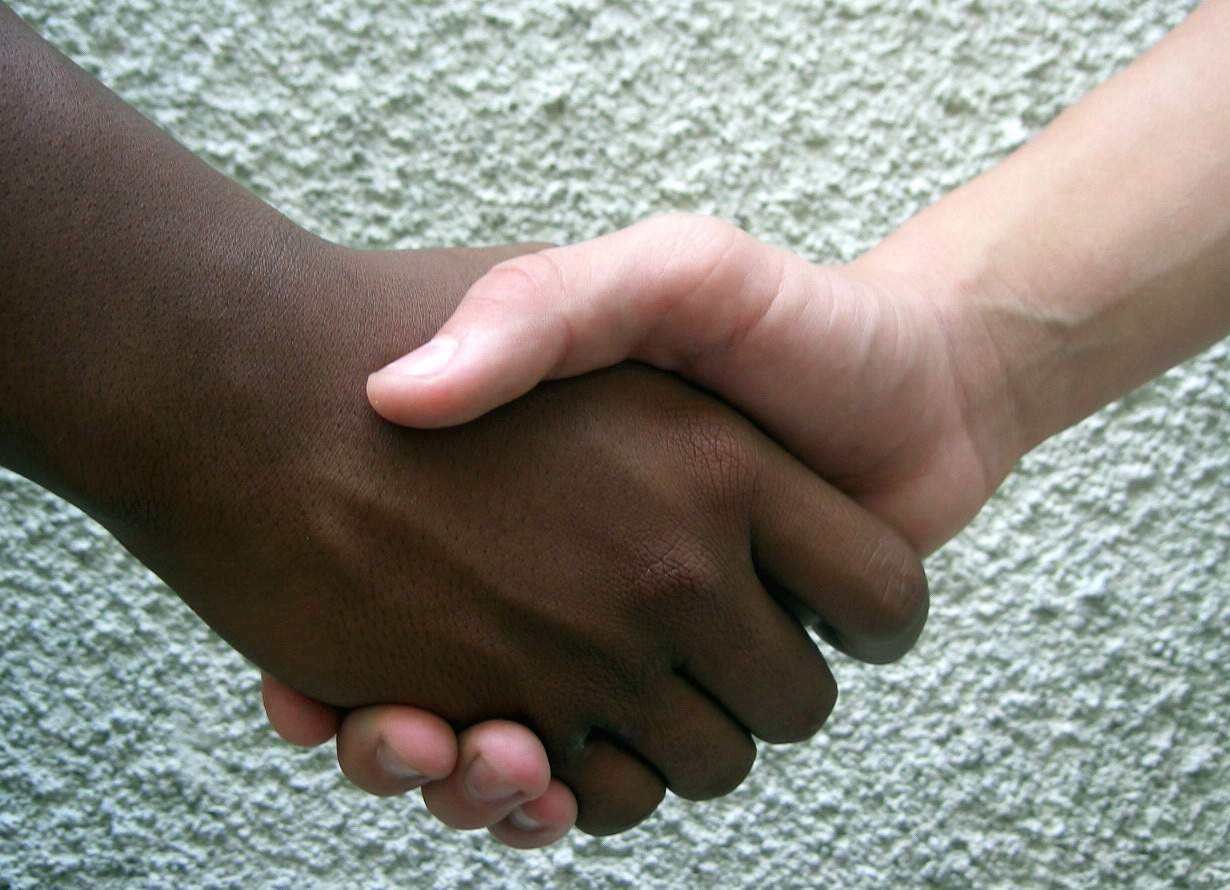
\includegraphics[width=3cm]{img/poignee.jpg}
\end{center}
On se pose la question suivante : « Quand $n$ personnes se rencontrent, si chacun serre la main des autres une seule fois, combien cela fait-il de poignées de main en tout ? ».\\
On décide de noter $f(n)$ ce nombre.
\begin{enumerate}[\bfseries 1.]
	\item 	\begin{enumerate}[\bfseries a.]
    	\item 	Que valent $f(2)$, $f(3)$, $f(4)$, $f(5)$ ?
    	\item 	Que valent logiquement $f(1)$ et $f(0)$ ?
    \end{enumerate}
	\item 	Supposons que l'on connaisse $f(10)$. Une 11\eme personne arrive. Combien doit-on ajouter à $f(10)$ pour obtenir $f(11)$ ?
    \item   Pour tout $n\in\N^*$, déduis-en ce que vaut $f(n)$ à partir de $f(n-1)$.
    \item   À partir du résultat précédent, écrit en \textsc{Python} la fonction \pythoninline{f} qui :
    \begin{enumerate}[--]
    	\item 	en entrée prend un \pythoninline{int n} positif;
    	\item 	renvoie le nombre de poignées de mains lors de la rencontre de \pythoninline{n} individus.
    \end{enumerate}
    \textbf{Indice :} rien n'interdit à \pythoninline{f} de «s'appeler elle-même» !
\end{enumerate}
\end{encadrecolore}

\begin{exercice}[]
	En s'inspirant de la fonction factorielle, coder en \textsc{Python} de manière récursive la fonction \pythoninline{somme} qui
	\begin{enumerate}[--]
		\item 	en entrée prend un entier naturel \pythoninline{n};
		\item 	renvoie zéro si \pythoninline{n} vaut zéro;
		\item 	renvoie \pythoninline{n + somme(n - 1)} sinon.
	\end{enumerate}
	On vérifiera que \pythoninline{somme(1000)} vaut \np{5050}. Expliquer ce que calcule \pythoninline{somme(n)}.
\end{exercice}

\begin{exercice}
Programmer la fonction \pythoninline{sommes_cubes()} en Python de manière récursive, et tester cette fonction.\\
\pythoninline{sommes_cubes(n)} devra renvoyer, pour $n\in\N$ $$\sum_{k=0}^nk^3$$ C'est-à-dire la somme des cubes des entiers naturels de 0 à $n$.
\end{exercice}

\begin{exercice}[ : récursion imbriquée]
	\vspace{1em}
	\begin{minipage}{10cm}
	La fonction $f_{91}$ de McCarthy est définie sur $\N$ par :
	$$f_{91}(n)=\begin{cases}
	n-10 & \mbox{si } n>100\\
	f_{91}\left(f_{91}(n+11)\right) &\mbox{sinon}
	\end{cases}$$
	Programmer $f_{91}$ en \textsc{Python} et vérifier que pour tout entier naturel $n$ inférieur ou égal à 101, $f_{91}(n)$ vaut... 91.
	\end{minipage}\hspace{1.5cm}\begin{minipage}{4.2cm}
		\begin{center}
			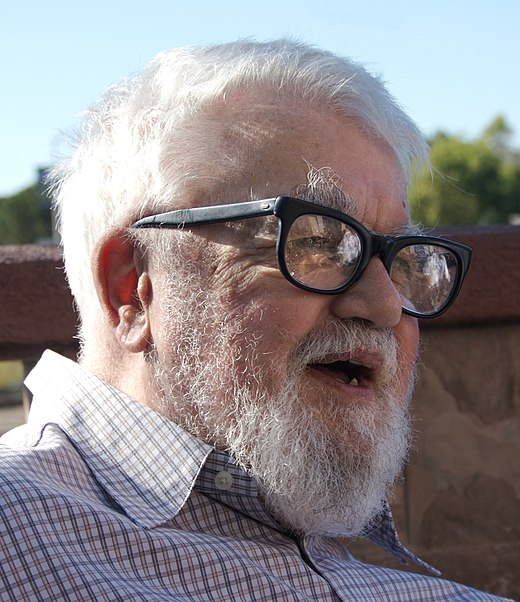
\includegraphics[width=4cm]{img/mccarthy}\\\scriptsize
			John McCarthy, informaticien, lauréat du prix Turing en 1971.
	\end{center}\end{minipage}\vspace{.5em}
\end{exercice}

\begin{exercice}[ : fonction puissance]
	Coder en \textsc{Python} la fonction \pythoninline{puissance} qui
	\begin{enumerate}[--]
		\item 	en entrée prend un \pythoninline{int} positif \pythoninline{n} et un \pythoninline{float x};
		\item 	renvoie la valeur de \pythoninline{x**n} calculée récursivement (cas de base et cas récursif à trouver soi-même).\end{enumerate}
\end{exercice}


\begin{exercice}[ : récursion mutuelle]
	On considère les deux suites $a$ et $b$ définie par
	$$a(n)=\begin{cases}
	1 & \mbox{si } n=0\\
	n-b(a(n-1)) &\mbox{sinon}
	\end{cases}
	\mbox{\hspace{3em} et\hspace{3em}}
	b(n)=\begin{cases}
	0 & \mbox{si } n=0\\
	n-a(b(n-1)) &\mbox{sinon}
	\end{cases}$$

	Programmer $a$ et $b$ en \textsc{Python}, puis conjecturer pour quelles valeurs de $n$ on a $a(n)\neq b(n)$ (ces valeurs sont en relation avec une suite déjà rencontrée).
\end{exercice}


\begin{exercice}[ : palindromes]
	Un \pythoninline{str} est un palindrome si on peut le lire à l'envers comme à l'endroit. Par exemple \og kayak\fg{}, \og  Un radar nu \fg{} ou \og !a!bcb!a!\fg{} sont des palindromes.\\
	\'Ecrire une fonction récursive \tw{palindrome} qui :
	\begin{enumerate}[--]
		\item 	en entrée prend un mot (un \pythoninline{str});
		\item 	renvoie \pythoninline{True} si c'est un palindrome et \pythoninline{False} sinon;
		\item 	procède récursivement
		\begin{enumerate}[\textbullet]
			\item 	si le mot a une lettre ou bien deux lettres pareilles, c'est un palindrome;
			\item 	sinon on regarde si les lettres du début et de la fin sont les mêmes. Si ce n'est pas le cas, ce n'est pas un palindrome. Si c'est le cas alors il faut regarder si le sous-mot restant est un palindrome.
		\end{enumerate}
	\end{enumerate}
	\textbf{Rappels :}
	Si \pythoninline{s} est un \pythoninline{str}
	\begin{enumerate}[--]
		\item 	\pythoninline{s[0]} et \pythoninline{s[-1]} sont respectivement son premier caractère et son dernier caractère.
		\item 	\pythoninline{s[p:q]} renvoie la sous chaîne allant de \pythoninline{s[p]} à \pythoninline{s[q-1]}.
	\end{enumerate}
\end{exercice}

\begin{exercice}[* : nombres de Catalan]
\vspace{1em}
\begin{minipage}{10cm}
Considérons l'opération \og puissance\fg{}. appliquée à trois nombres, par exemple 2, 3 et 4, pris dans cet ordre. Il y a plusieurs manière de
procéder :
\begin{itemize}
	\item	$2^{(3^4)}=2^{81}=2 417 851 639 229 258 349 412 352$
	\item 	$(2^3)^4 = 8^4=4096$
\end{itemize}
Pour 3 nombres, il y a donc 2 manières de placer les parenthèses pour effectuer les opérations.\\
Et pour 4 nombres ? Pour 5 ?
Pour simplifier l’écriture on peut noter $a*b$ au lieu de $a^b$. \\
Alors avec $n$ lettres on peut reformuler l’exemple précédent ainsi
: quel est le nombre de manières (noté $C_n$) de placer des parenthèses autour des lettres de sorte que
\end{minipage}\hspace{1.5cm}\begin{minipage}{4.2cm}
\begin{center}
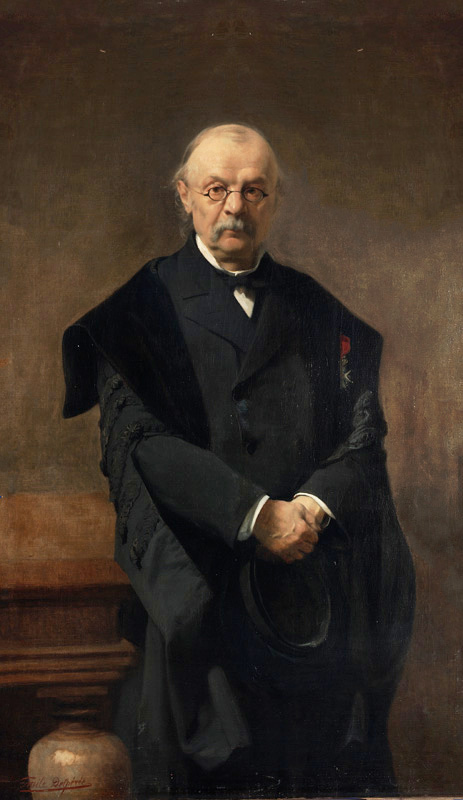
\includegraphics[width=4cm]{img/catalan}\\\scriptsize
Eugène Catalan, mathématicien franco-belge du \textsc{xix}\eme siècle.
\end{center}\end{minipage}\vspace{.5em}

\begin{enumerate}[--]
	\item 	on n'ait jamais plus de deux termes non parenthésés : pas de choix à faire ;
	\item 	on ne mette jamais des parenthèses autour d’un seul terme : pas de parenthèses inutiles.
\end{enumerate}
Les premiers cas sont simples :

\begin{enumerate}[\textbullet]
	\item 	$C_1=1$ : il n'y a qu'une manière d'écrire $a$.
	\item 	$C_2=1$ aussi : une seule possibilité : $a*b$.
	\item 	$C_3=2$, on l'a vu : $a*(b*c)$ et $(a*b)*c$.
	\item 	Pour calculer $C_4$, on peut classer les parenthésages suivant la dernière opération $*$ à faire :
	\begin{itemize}
		\item 	après $a$ : il y a $a*((b*c)*d)$ et $a*(b*(c*d))$.
		\item 	\og entre $b$ et $c$\fg{} : $(a*b)*(c*d)$.
		\item 	juste avant $d$ : $((a*b)*c)*d$ et $(a*(b*c))*d$.
	\end{itemize}
	Finalement cela fait 5 possibilités, $C_4=5$ et on remarque que $C_4=C_1C_3+C_2C_2+C_3C_1$.
\end{enumerate}
Cela se généralise : pour tout $n$ entier supérieur à 2 on a
$$C_n=C_1C_{n-1}+C_2C_{n-2}+\ldots+C_{n-1}C_1$$
En effet, on commence par choisir la position de la dernière opération à effectuer : puisqu'il y a $n$ lettres il y a $n-1$ choix de positions
possibles, chacun scindant le mot de $n$ lettres en un mot de $p$ lettres et un autre de $n-p$, qui donnent donc lieu respectivement à $C_p$ et
$C_{n-p}$ parenthésages indépendants, donc $C_pC_{n-p}$ parenthésages en tout. En considérant toutes les valeurs de $p$ possibles on arrive à
\begin{equation}
\tag{*}
C_n=\sum_{p=1}^{n-1}C_pC_{n-p}
\label{eqn:Catalan}
\end{equation}

Ce qui permet de calculer $C_5 =14$, $C_6 =42$, $C_7 =132$, $C_8 =429$, $C_9 =1430$, $C_{10} =4862$...\\

\textbf{Travail à faire :}\\

Programmer la fonction \pythoninline{catalan} en \textsc{Python} :
\begin{enumerate}[--]
	\item 	Le cas de base est pour \pythoninline{n} valant \pythoninline{1}, où la fonction renvoie \pythoninline{1};
	\item 	Si \pythoninline{n} est plus grand, alors on calcule \pythoninline{catalan(n)} récursivement à l'aide de \eqref{eqn:Catalan}.
\end{enumerate}

On pourra utiliser la fonction \tw{sum}.\\
Par exemple \pythoninline{sum(n for n in range(10))} calcule la somme $0+1+...+9$.
\end{exercice}

%-------------------------------------
\newpage
{\huge\titlefont\color{subsection@color} Exercices supplémentaires}
\begin{exercice}[ : approximation d'un flocon de Von Koch]
	On part d'un segment (étape 0) que l'on coupe en 3 parties égales. Sur le segment du milieu on construit un triangle équilatéral puis on enlève ce segment. On obtient alors une itération du procédé de Von Koch. On peut ensuite répéter indéfiniment ce procédé.
	\begin{center}
		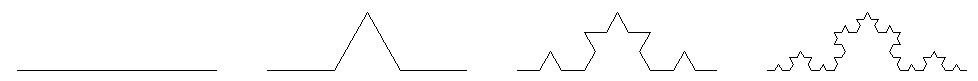
\includegraphics[width=16cm]{img/koch}\\
		\scriptsize Les 4 premières étapes du procédé.
	\end{center}
	Lorsque l'on part d'un triangle équilatéral auquel on applique ce procédé une infinité de fois, l'objet obtenu s'appelle un \textit{flocon de Von Koch}. Il a la particularité d'avoir une aire finie mais un périmètre infini.
	\begin{center}
					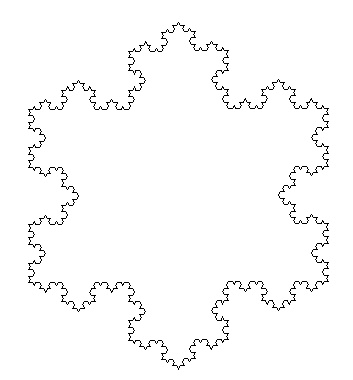
\includegraphics[width=6cm]{img/flocon}\\
		\scriptsize Une approximation d'un flocon de Von Koch.
	\end{center}
Pour dessiner, on va utiliser le module \pythoninline{turtle} de \textsc{Python}.
\begin{enumerate}[\bfseries 1.]
	\item  Regarde bien le micro-tutoriel pour comprendre le fonctionnement de base de \pythoninline{turtle}.
	\item 	Coder la fonction \pythoninline{koch} qui
		\begin{enumerate}[--]
			\item 	en entrée prend un \pythoninline{float x} (longueur du segment de base) et un \pythoninline{int n} (nombre d'itérations);
			\item 	ne renvoie aucune valeur mais dessine le processus itéré n fois, de manière récursive.
		\end{enumerate}
\end{enumerate}
\end{exercice}

\begin{exercice}[ : fonction puissance améliorée]
	Soit $x$ un nombre réel et $n$ un entier positif alors on a \\
		$$x^n=\begin{cases}
	(x^{n/2})^2 & \mbox{si } n \mbox{ est pair}\\
	x\times(x^{(n-1)/2})^2 &\mbox{sinon}
	\end{cases}$$
	\begin{enumerate}[\bfseries 1.]
		\item 	En se basant sur cette observation, coder une fonction \pythoninline{puissance_amelioree} qui a les mêmes spécifications que la fonction \pythoninline{puissance} vue dans un exercice précédent.
		\item 	Créer pour ces deux fonctions une variable \pythoninline{nb_appels} pour comptabiliser le nombre d'appels récursifs et comparer ces nombres dans \pythoninline{puissance(2,128)} et \pythoninline{puissance_amelioree(2,128)}.
	\end{enumerate}
\end{exercice}
\begin{exercice}[ : algorithme d'Euclide récursif]
	Soient $n$ et $p$ deux entiers strictement positifs. On note $\mbox{pgcd}(a;b)$ le plus grand entier qui divise à la fois $a$ et $b$.\\
	Par exemple
	\begin{enumerate}[--]
		\item 	$1050 = 2\times 3\times	5\times 5\times 7$;
		\item 	$770=2\times 5\times 7\times 11$;
		\item 	le pgcd de ces deux nombres est donc $2\times 5\times 7 =70$.
	\end{enumerate}
	Pour trouver le pgcd de deux nombres on peut, comme dans l'exemple précédent, les décomposer en produit de facteurs premiers et prendre le produit de tous les facteurs communs, mais on peut aussi utiliser l'algorithme d'Euclide :\\
	Soient $a$ et $b$ deux entiers strictement positifs, on suppose que $a\leqslant b$
	\begin{enumerate}[--]
		\item on écrit la division euclidienne de $a$ par $b$ : $a=q\times b + r$ avec $r<b$;
		\item si un entier divise $a$ et $b$ alors on peut facilement montrer qu'il divise aussi $r$, de sorte que $\mbox{pgcd}(a;b)=\mbox{pgcd}(b;r)$.
		\item si $r\neq 0$ alors on recommence alors en prenant $a$ égal à $b$ et $b$ égal à $r$;
		\item si $r=0$ alors le pgcd des nombres de départ est le dernier $b$ qu'on a utilisé.
	\end{enumerate}
	Voyons la méthode sur un exemple :
	\begin{enumerate}[--]
		\item 	on divise $1050$ par $280$ : $1050 = 1\times 770 + 280$
		\item 	on divise $770$ par $280$ : $770 = 2\times 280 + 210$
		\item 	on divise $280$ par $210$ : $280 = 1\times 210 + 70$
		\item 	on divise $210$ par $70$ : $210 = 3\times 70 + 0$
		\item 	le reste est nul, le dernier diviseur est 70 et c'est le pgcd des deux nombres de départ.
	\end{enumerate}
	Programmer cette fonction \pythoninline{pgcd} de manière récursive.
\end{exercice}
\end{document}
